\documentclass[12pt,letterpaper]{scrartcl}
\usepackage{lipsum}
\usepackage[utf8]{inputenc}
\usepackage{amsmath}
\usepackage{amsfonts}
\usepackage{amssymb}
\usepackage{graphicx}
\usepackage[left=3cm,right=2.5cm,top=2.5cm,bottom=2.5cm]{geometry}
\usepackage[ruled]{algorithm2e}
\author{Don cuyi}

\newcommand{\A}[1]{A_{#1}}
%\cof{11}{\alpha}{0}{\alpha}{-\beta}

%Color
\usepackage{color}
\definecolor{nred}{RGB}{174,49,54}
\definecolor{nblue}{RGB}{86,99,146}
\definecolor{nalgo}{RGB}{188,139,76}
\usepackage{sectsty}
\sectionfont{\color{nred}}
\subsectionfont{\color{nblue}}
\subsubsectionfont{\color{nalgo}}

%Librías tikz
\usepackage{pgf,tikz}
\usepackage{mathrsfs}
\usetikzlibrary{arrows}
\usetikzlibrary[patterns]
\newcommand{\degre}{\ensuremath{^\circ}}
\definecolor{qqwuqq}{rgb}{0.,0.39215686274509803,0.}
\definecolor{ffttww}{rgb}{1.,0.2,0.4}
%Hipervinculos
\usepackage{hyperref}

\usepackage{fancyhdr}
\pagestyle{fancy}
\fancyhf{}
\fancyhead[L]{}
\fancyhead[C]{Licenciatura en ciencia de la computación}
\fancyhead[R]{USACH}

%interlineado
\renewcommand{\baselinestretch}{1.2}

%\bibitem{Yahoo} \textsc{Andres G} (2009),
%\textbf{¿Generar números aleatorios negativos en Lenguaje C?} En \textsc{Yahoo! respuestas}
%Recuperado el el 23 del julio del 2014
%\url{https://es.answers.yahoo.com/question/index?qid=20091121055249AAUQH3N}

\newcommand{\biblio}[7]{
\bibitem{#1} \textsc{#2} (#3),
\textbf{#4} En \textsc{#5}
Recuperado el #6
\url{#7}
}

% Last, F. M. (Year Published) Book. City, State: Publisher.
\newcommand{\book}[5]{
\bibitem{#1} \textsc{#2} (#3),
\textbf{#4}  \textsc{#5} Estado: Publicado
}

\begin{document}

\begin{titlepage}

\begin{center}

{\Large { Licenciatura en ciencia de la computación} }


\includegraphics[scale=1]{UDSCNRJ}
\\[1cm]

{\Huge \textsc{Algoritmo de Strassen}}\\[0.7cm]

{\huge Complejidad}\\[2cm]


\begin{minipage}[l]{0.4\textwidth}
	\begin{flushleft}
	\linespread{1}
		\textbf{\textsf{Profesor:}}\\
		\large Nicolas Thériault
	\end{flushleft}
\end{minipage}
\begin{minipage}[l]{0.4\textwidth}

	\begin{flushright}

		\textbf{\textsf{Autor:}}\\
		\linespread{1}
		\large Sergio Salinas\\
		\large Danilo Abellá\\

	\end{flushright}
\end{minipage}

\end{center}

\end{titlepage}



\newpage

\tableofcontents

\newpage
\section{Introducción}

Este informe trata sobre el algoritmos de multiplicación de Strassen, se verá su demostración, su complejidad y la de la multiplicación normal y se verá su eficiencia.

Los programas fueron escritos en lenguaje C usando el compitalador GCC versión 5.4.

\section{Análisis teorico}

\subsection{Demostración Strassen}
Dada la multiplicación de dos matrices  A y B
$$
AB =
\begin{pmatrix}
A_{11} & A_{12} \\
A_{21} & A_{22}\\
\end{pmatrix}
\begin{pmatrix}
B_{11} & B_{12} \\
B_{21} & B_{22}\\
\end{pmatrix}
 = \begin{pmatrix}
A_{11} B_{11} + A_{12} B_{21} & A_{11} B_{12} + A_{12} B_{22}\\
A_{21} B_{11} + A_{22} B_{21} & A_{21} B_{12} + A_{22} B_{22}\\
\end{pmatrix}
=
\begin{pmatrix}
C_{11} & C_{12} \\
C_{21} & C_{22}\\
\end{pmatrix}
$$

Se calculan los S y los T de la técnica de Strassen.


\[
\begin{array}{lcl}
	S_1 &=& A_{21} + A_{22} \\
	S_2 &=& A_{21} + A_{22} - A_{11} \\
	S_3 &=& A_{11} - A_{21}\\
	S_4 &=& A_{12} -A_{21} - A_{22} + A_{11} \\
\end{array}
\]

\[
\begin{array}{lcl}
	T_1 &=& B_12 - B_{11}\\
	T_2 &=& B_{22} - B_{12} + B_{11}\\
	T_3 &=& B_{22} - B_{12}\\
	T_4 &=& B_{22} - B_{12} + B_{11} - B_{21}\\
\end{array}
\]
Se calculan los P.
\[
\begin{array}{lcl}
	P_1 &=& A_{11}B_{21}\\
	P_2 &=& A_{12}B_{21}\\
	P_3 &=& A_{12}B_{22} - A_{21}B_{22} - A_{22}B_{22} + A_{11}B_{22}\\
	P_4 &=& A_{22}B_{22} - A_{22}B_{12} + A_{22}B_{11}  - A_{22}B_{21}\\
	P_5 &=& A_{21}B_{11} - A_{21}B_{11} + A_{22}B_{12}- A_{22}B_{11}\\
	P_6 &=& A_{21}B_{22} - A_{21}B_{12} + A_{21}B_{11} + A_{22}B_{22} - A_{22}B_{12} + A_{22}B_{11} - A_{11}B_{22}+ A_{11}B_{22}\\
	&&  + A_{11}B_{12} - A_{11}B_{11}\\
	P_7 &=& A_{11}B_{22} - A_{11}B_{12} - A_{21}B_{22} + A_{21}B_{12}\\
\end{array}
\]
Se calculan los U
\[
\begin{array}{lcl}
	U_{1} &=& A_{11}B_{11} + A_{12}B_{21}\\
	U_{2} &=& A_{21}B_{22} - A_{21}B_{12} + A_{21}B_{11} + A_{22}B_{22} - A_{22}B_{12} + A_{22}B_{11} - A_{11}B_{22} + A_{11}B_{12}\\
	U_{3} &=& A_{21}B_{11} + A_{22}B_{22} - A_{22}B_{12} + A_{22}B_{11}\\
	U_{4} &=& A_{21}B_{22} + A_{22}B_{22} - A_{11}B_{22} + A_{11}B_{12}\\
	U_{5} &=& A_{11}B_{12} + A_{12}B_{22}\\
	U_{6} &=& A_{21}B_{11} + A_{22}B_{21}\\
	U_{7} &=& A_{22}B_{22} + A_{21}B_{12}\\
\end{array}
\]

De está forma se obtiene que

$$
A\cdot B =
\begin{pmatrix}
	U_1 & U_5\\
	U_6 & U_7\\
\end{pmatrix}
 = \begin{pmatrix}
A_{11} B_{11} + A_{12} B_{21} & A_{11} B_{12} + A_{12} B_{22}\\
A_{21} B_{11} + A_{22} B_{21} & A_{21} B_{12} + A_{22} B_{22}\\
\end{pmatrix}
=
\begin{pmatrix}
C_{11} & C_{12} \\
C_{21} & C_{22}\\
\end{pmatrix}
$$

Con  lo que se demuestra que el algoritmo de strassen es equivalente a la multiplicación de matrices.

\subsection{Análisis complejidad}

\subsubsection{Strassen}

Strassen hace en total 7 multiplicaciones más 14 sumas (y restas, aunque se tratan como su fueran la misma operación) y además divide el orden de la matriz en dos por cada recurrencia por lo su relación de recurrencia es

$$ T(n) = 7 \cdot T \left ( \dfrac{n}{2} \right ) + 14n^2 $$

Dado el teorema maestro se obtiene que $a = 7$, $b = 2$ y $d = 2$, obteniendo que $7 > 2^2$ por que la complejidad del algoritmos es

$$T(n) \in O(n^{\log_2 7}) = O ( n^{2.80735} )$$

\subsubsection{Multiplicación clásica}

%http://www.lcc.uma.es/~av/Libro/CAP3.pdf
La multiplicación clásica de matrices cuadradas de orden 2 debe hacer un total de 8 multiplicaciones escalares y 4 sumas de coste $n^2$, por lo que si quiere trabajar con bloques de matrices cuadradas de orden $n = 2^k$ el total de multiplicaciones tendría como relación de recurrencia:

$$ T(2^k) = 8\cdot T( 2^{k-1}) + 4(2^k)^2 $$

Usando el teorema maestro se obtiene que la complejidad de la multiplicaciones es

$$T(n) \in O(n^{\log_2 8}) = O ( n^{3} )$$

Lo que es consistente con el costo $n^3M + (n^3 - n^2)A$.

\subsection{Valor de $\mathbf{n_0}$}

Después de probar con varias potencias de 2 se pudo concluir que el punto en donde Strassen lleva ventaja por sobre la multiplicación clásica es en $n_0$ = 16. 

Esto es debido a que en los valores menores y mayores a 16 se puede apreciar dos rectas continuas con crecimiento distinto, mientras que cuando $n_0$ vale 16 se pueden ver los resultados como una sola recta.


\section{Algoritmos Desarrollados}

\begin{algorithm}[H]
 \KwData{Dos matrices A y B de orden n, $n_0$}
 \KwResult{Matriz C}
 \eIf{n $\leq$ $n_0$}{ A$\cdot$B\;}{
	Dividir A en $A_{11}$, $A_{12}$, $A_{21}$ y $A_{22}$\;
	Dividir B en $B_{11}$, $B_{12}$, $B_{21}$ y $B_{22}$\;
	
$S_1 \leftarrow A_{21} + A_{22}$; $\,$  $T_1 \leftarrow  B_{12} - B_{11}$\;  
$S_2 \leftarrow  S_{1} -  A_{11}$; $\;$ $T_2 \leftarrow  B_{22} - T_{1}$\;
$S_3 \leftarrow  A_{11} - A_{21}$;  $T_3 \leftarrow  B_{22} - B_{12}$\;
$S_4 \leftarrow  A_{12} - S_{2}$; $\;$  $T_4 \leftarrow  T_{2} -  B_{21}$\;


 \eIf {n/4 $\leq$ $n_0$ }{
$ P_1  \leftarrow A_{11}\cdot B{11}$;
$ P_2  \leftarrow A_{12}\cdot B{21}$\;
$ P_3  \leftarrow S_{4}\cdot B{22}$;
$ P_4  \leftarrow A_{22}\cdot T{4}$\;
$ P_5  \leftarrow S_{1}\cdot T{1}$;
$ P_6  \leftarrow S_{2}\cdot T{2}$\;
$ P_7  \leftarrow S_{3}\cdot T{3}$;
}{
$ P_1  \leftarrow strassen(A_{11} ,B{11},n, n_0  )$\;
$ P_2  \leftarrow strassen(A_{12} ,B{21},n, n_0  )$\;
$ P_3  \leftarrow strassen(S_{4} ,B{22},n, n_0  )$\;
$ P_4  \leftarrow strassen(A_{22}, T{4},n, n_0  )$\;
$ P_5  \leftarrow strassen(S_{1}, T{1},n, n_0  )$\;
$ P_6  \leftarrow strassen(S_{2}, T{2},n, n_0  )$\;
$ P_7  \leftarrow strassen(S_{3}, T{3},n, n_0  )$	\;
}
$U_1  \leftarrow P_1 + P_2$\;
$U_2  \leftarrow P_1 + P_6$\;
$U_3  \leftarrow U_2 + P_7$\;
$U_4  \leftarrow U_2 + P_5$\;
$U_5  \leftarrow U_4 + P_3$\;
$U_6  \leftarrow U_3 - P_4$\;
$U_7  \leftarrow U_3 + P_5$\;
}
return $C \leftarrow \begin{pmatrix}
	U_1 & U_5\\
	U_6 & U_7\\
\end{pmatrix}$
 \caption{\textbf{Strassen}. Multiplica dos matrix A y B}

\end{algorithm}
\newpage
\begin{algorithm}[H]
 \KwData{Dos matrices A y B de largo n}
 \KwResult{La matrix C con la multiplicación de A y  B}
 \For{i $\leftarrow$ 0 ... n-1}{
	 \For{j $\leftarrow$ 0 ... n-1}{
		 $C_{ij} \leftarrow 0$\;
			 \For{k $\leftarrow$ 0 ... n-1}{
			 	$C_ij \leftarrow C_{ij} + A_{ik} \cdot B_{kj}$
 } 	
 }
 }
 \caption{\textbf{Multiply Matrix}. Multiplica dos matrices A y B}
\end{algorithm}

\begin{algorithm}[H]
 \KwData{Dos matrices A y B de largo n}
 \KwResult{La matrix C con la suma de A y  B}
 \For{i $\leftarrow$ 0 ... n-1}{
	 \For{j $\leftarrow$ 0 ... n-1}{
		$C_ij \leftarrow A_{ij} + B_{ij} $
 } 	
 }
  \caption{\textbf{Sum Matrix}. Suma dos matrices A y B}
\end{algorithm}

 \begin{algorithm}[H]
 \KwData{Dos matrices A y B de largo n}
 \KwResult{La matrix C con la resta de A y  B}
 \For{i $\leftarrow$ 0 ... n-1}{
	 \For{j $\leftarrow$ 0 ... n-1}{
		$C_ij \leftarrow A_{ij} - B_{ij} $
 } 	
 }
 
 \caption{\textbf{Sub Matrix}. Resta dos matrices A y B}
\end{algorithm}

\newpage



\section{Información de Hardware y Software}


\subsection{ Notebook - Danilo Abellá}
\subsubsection{Software}
\begin{itemize}
\item SO: Xubuntu 16.04.1 LTS
\item GMP Library
\item Mousepad 0.4.0
\end{itemize}

\subsubsection{Hardware}
\begin{itemize}
\item AMD Turion(tm) X2 Dual-Core Mobile RM-72 2.10GHz
\item Memoria (RAM): 4,00 GB(3,75 GB utilizable)
\item Adaptador de pantalla: ATI Raedon HD 3200 Graphics
\end{itemize}



\subsection{Notebook - Sergio Salinas}
\subsubsection{Software}
\begin{itemize}
\item  SO: ubuntu Gnome 16.04 LTS
\item Compilador: gcc version 5.4.0 20160609
\item Editor de text: Atom
\end{itemize}

\subsubsection{Hardware}
\begin{itemize}
\item Procesador: Intel Core i7-6500U CPU  2.50GHz x 4
\item Video: Intel HD Graphics 520 (Skylake GT2)
\end{itemize}
\newpage



\section{Curvas de desempeño de resultados}

\subsection{Multiplicación clasica vs distintos valores de $\mathbf{n_0}$}
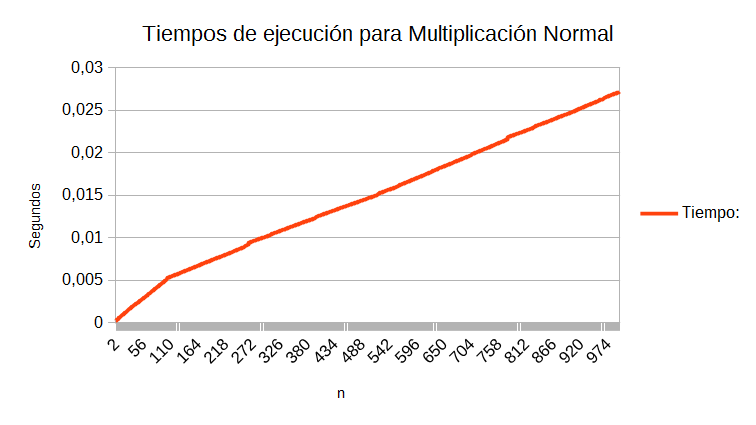
\includegraphics[scale=0.6]{normal.png} 

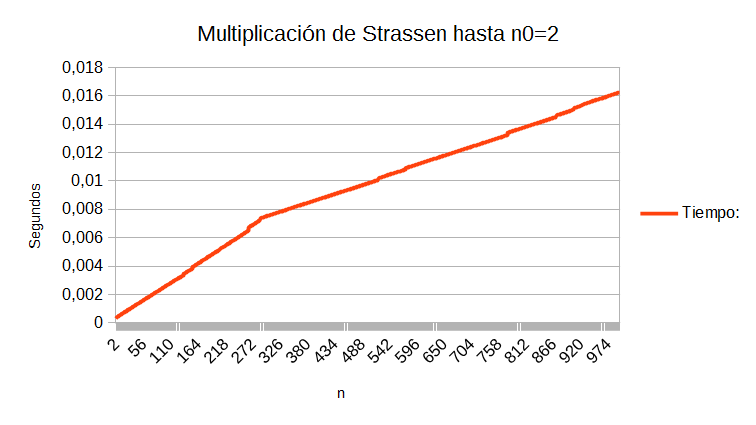
\includegraphics[scale=0.6]{n0-2.png} 

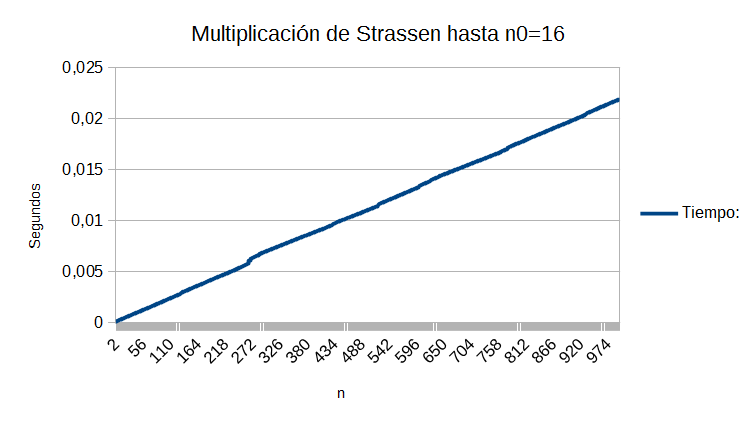
\includegraphics[scale=0.6]{n0-16.png} 

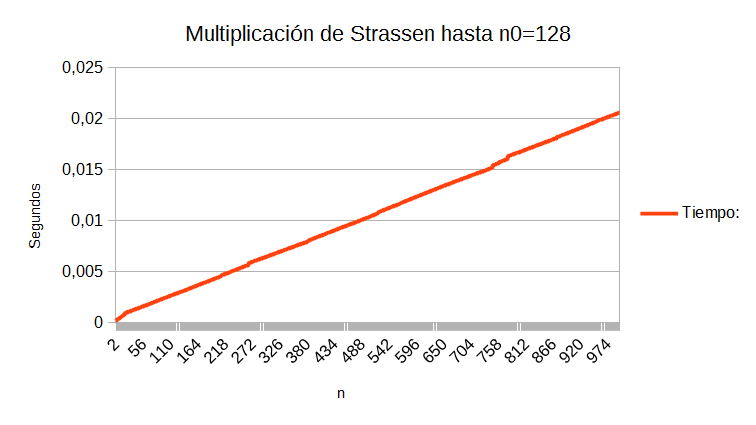
\includegraphics[scale=0.6]{n0-128.png} 

\subsection{$\mathbf{n_0}$ = 16*k, k=\{1,2 ... 16\}}

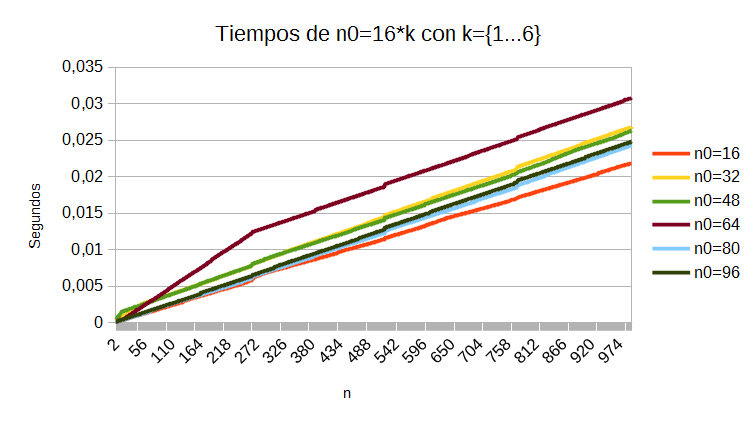
\includegraphics[scale=0.6]{1-6.png} 

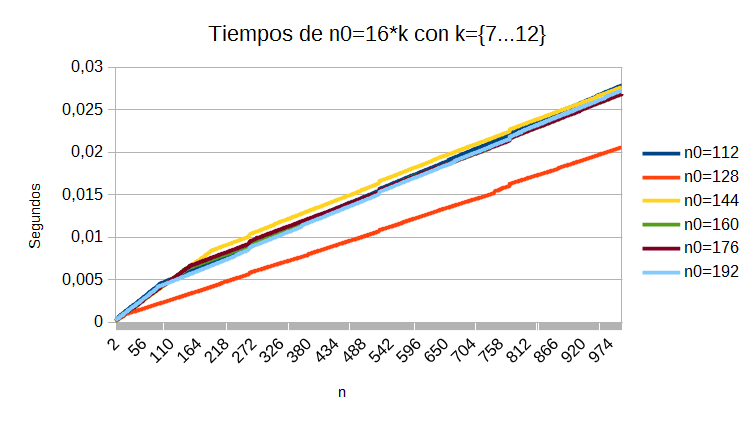
\includegraphics[scale=0.6]{7-12.png} 

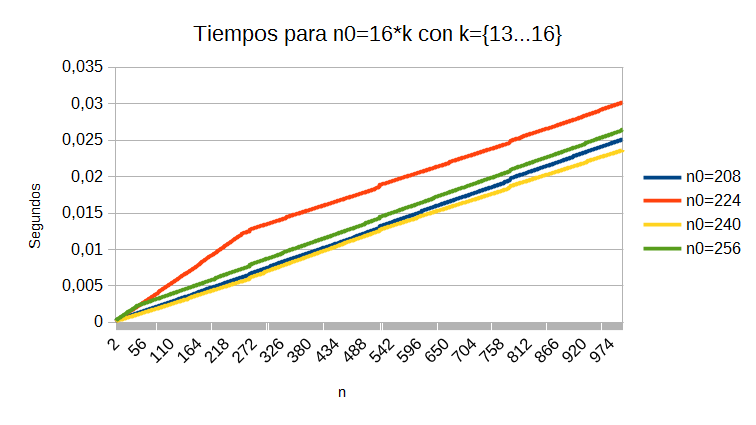
\includegraphics[scale=0.6]{13-16.png} 
\newpage
\section{Conclusiones}

Se puede concluir que la eficiencia de la multiplicación de Strassen ($O(n^{2.801}$)) por sobre la clásica ($O(n^{3})$) es indiscutible, llegando está última incluso a tomar el doble de tiempo que Strassen cuando aunque la última es más eficiente cuando se trata de matrices de orden estrictamente menores a 16.

\end{document}
